\section{Covariant Derivative}

If we want to give a one-sentence definition of the  Covariant Derivative, we can
say it's the \textbf{understanding the rate of change of vector (tensor) fields
that takes changing basis vectors into account}

There's obviously some explanation and proof required, and we're going to define the 
Covariant Derivative first in the flat space, which is the easiest way to look at it, 
and then follow along, increasing the challenge, by looking at it in curved-space, first extrinsic and 
then intrinsic, and finally giving its most abstract definition.\\

\subsection{Covariant derivate in flat-space}

Let's start by recalling that, given a certain basis, we can define a vector $\color{orange}\vec{v}$ as a 
linear conbination of the basis vectors, for example in cartesian basis $\color{blue}\vec{e_i}$ or polar $\color{red}\tilde{\vec{e_j}}$:

\begin{align*}
    \begingroup\color{orange}\vec{v}\endgroup = \begingroup\color{cyan}v^i\endgroup \begingroup\color{blue}\vec{e_i}\endgroup\\
    \begingroup\color{orange}\vec{v}\endgroup = \begingroup\color{magenta}v^i\endgroup \begingroup\color{red}\tilde{\vec{e_i}}\endgroup
\end{align*}

If we try to differentiate the vector with respect to one of the coordinates in cartesian basis in $\mathbb{R}^2$, let's say x:

\begin{align*}
    \frac{\partial}{\partial \begingroup\color{cyan}x\endgroup} (\begingroup\color{orange}\vec{v}\endgroup) &= 
    \frac{\partial}{\partial \begingroup\color{cyan}x\endgroup} \left(\begingroup\color{cyan}v^x\endgroup \begingroup\color{blue}\vec{e_x}\endgroup + \begingroup\color{cyan}v^y\endgroup \begingroup\color{blue}\vec{e_y}\endgroup\right)\\ &=
    \frac{\partial}{\partial \begingroup\color{cyan}x\endgroup} \left(\begingroup\color{cyan}v^x\endgroup \begingroup\color{blue}\vec{e_x}\endgroup\right) + \frac{\partial}{\partial \begingroup\color{cyan}x\endgroup} \left(\begingroup\color{cyan}v^y\endgroup \begingroup\color{blue}\vec{e_y}\endgroup\right)\\ &=
    \frac{\partial \begingroup\color{cyan}v^x\endgroup}{\partial \begingroup\color{cyan}x\endgroup} \begingroup\color{blue}\vec{e_x}\endgroup + \begingroup\color{cyan}v^x\endgroup \cancel{\frac{\partial}{\partial \begingroup\color{cyan}x\endgroup} \left(\begingroup\color{blue}\vec{e_x}\endgroup\right)}
    + \frac{\partial \begingroup\color{cyan}v^y\endgroup}{\partial \begingroup\color{cyan}x\endgroup} \begingroup\color{blue}\vec{e_y}\endgroup + \cancel{\begingroup\color{cyan}v^y\endgroup \frac{\partial}{\partial \begingroup\color{cyan}x\endgroup} \left(\begingroup\color{blue}\vec{e_y}\endgroup\right)}\\
    &= \frac{\partial \begingroup\color{cyan}v^x\endgroup}{\partial \begingroup\color{cyan}x\endgroup} \begingroup\color{blue}\vec{e_x}\endgroup + \frac{\partial \begingroup\color{cyan}v^y\endgroup}{\partial \begingroup\color{cyan}x\endgroup} \begingroup\color{blue}\vec{e_y}\endgroup
\end{align*}

where the canceled components are due to the fact that, in cartesian coordinates, the basis vectors are just constant, so the derivative is reduced to be 
a linear combination of the basis vectors, with coefficients given by the derivative of the vector components.\\

Different is the case of polar coordinates though, because the vector basis are not constant in space, but change from point to poing.
In polar coordinates, we end up with 4 components, 2 of them track the rate of change of components, and 2 of them track the change of the basis vectors.\\

In general, this is actually the simplest definition of the covariant derivative, so an ordinary derivative 
that takes into account the change of basis, so it makes sure to differentiate both the components and the basis vectors.\\
Writing that down using Einstein summation convention:

\begin{align*}
    \frac{\partial}{\partial \begingroup\color{cyan}c^i\endgroup} (\begingroup\color{orange}\vec{v}\endgroup) &= 
    \frac{\partial}{\partial \begingroup\color{cyan}c^i\endgroup} \left(\begingroup\color{cyan}v^j\endgroup \begingroup\color{blue}\vec{e_j}\endgroup\right)\\
    &= \frac{\partial \begingroup\color{cyan}v^j\endgroup}{\partial \begingroup\color{cyan}c^i\endgroup} \begingroup\color{blue}\vec{e_j}\endgroup
    + \begingroup\color{cyan}v^j\endgroup \frac{\partial \begingroup\color{blue}\vec{e_j}\endgroup}{\partial \begingroup\color{cyan}c^i\endgroup}
\end{align*}

Sometimes, the basis vector derivative, is commonly expanded into a linear combination of the basis 
vectors themselves, so:

\begin{align*}
    \frac{\partial \begingroup\color{blue}\vec{e_j}\endgroup}{\partial \begingroup\color{cyan}c^i\endgroup} &= 
    \begingroup\color{cyan}\Gamma^1_{ij}\endgroup \begingroup\color{blue}\vec{e_1}\endgroup + \begingroup\color{cyan}\Gamma^2_{ij}\endgroup \begingroup\color{blue}\vec{e_2}\endgroup\\
    &= \begingroup\color{cyan}\Gamma^k_{ij}\endgroup \begingroup\color{blue}\vec{e_k}\endgroup
\end{align*}

So the covariant derivative can be re-written as:

\begin{align*}
    \frac{\partial}{\partial \begingroup\color{cyan}c^i\endgroup} (\begingroup\color{orange}\vec{v}\endgroup) &= 
    \frac{\partial \begingroup\color{cyan}v^k\endgroup}{\partial \begingroup\color{cyan}c^i\endgroup} \begingroup\color{blue}\vec{e_k}\endgroup
    + \begingroup\color{cyan}v^j\endgroup \begingroup\color{cyan}\Gamma^k_{ij}\endgroup \begingroup\color{blue}\vec{e_k}\endgroup\\
    &= \left(\frac{\partial \begingroup\color{cyan}v^k\endgroup}{\partial \begingroup\color{cyan}c^i\endgroup} + \begingroup\color{cyan}v^j\endgroup \begingroup\color{cyan}\Gamma^k_{ij}\endgroup\right)\begingroup\color{blue}\vec{e_k}\endgroup
\end{align*}

\subsection{Covariant derivate in curved-space - extrinsic}

So now we're moving on into looking at the rate of change of vector fields, on curved surfaces.\\
It turns out that it's a lot trickier dealing with vector spaces here, when compared to flat ones, and we're going to explain why.

Let's take these two vector fields here below, you can clearly visualize that the first one is constant, whereas the second one is not:

\begin{center}
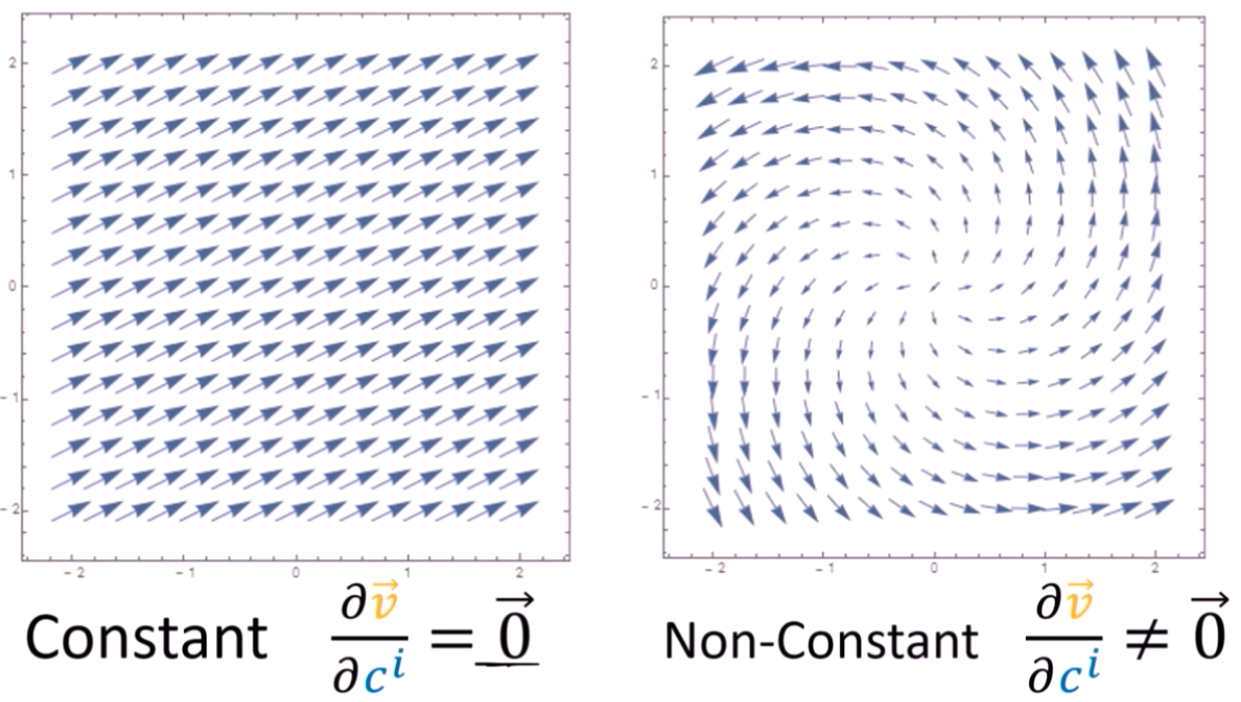
\includegraphics[scale=0.2]{figures/constant-vs-non-constant-vf.png}
\end{center}

The first one is constant because we can see that all the vectors are the same...but how do we say that?
It may sounds silly and straight forward, but how do we know that these are the same? Well what we could do is take
a couple of these vectors shown in the first picture, and slide one on top of the other, and check if they overlap perfectly. That's quite
easy to do right?\\

But let's consider instead, a vector field existing on the surface of a 2D sphere, so every point on the sphere, has 
a vector associated to it. And now let's try to ask the same question: if we compare the blue vector and the red vector in the picture, 
how do we tell if they're the same?

\begin{center}
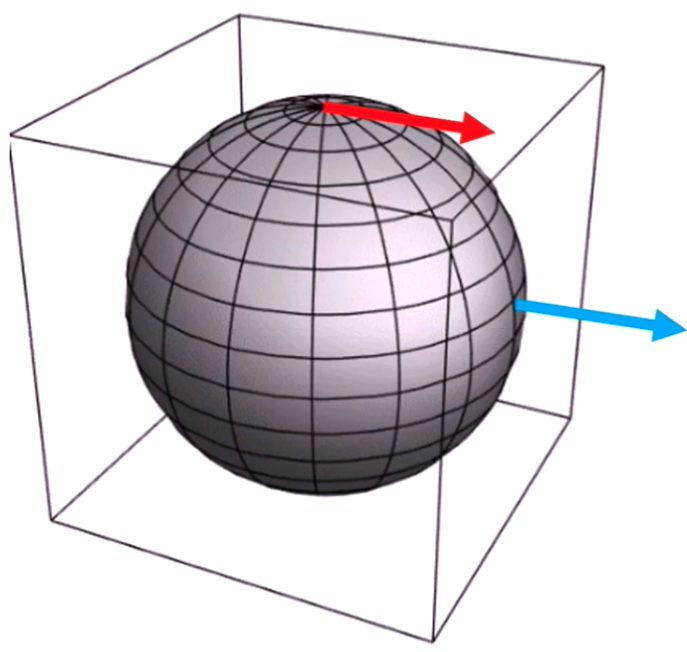
\includegraphics[scale=0.2]{figures/vector-comp-sphere.png}
\end{center}

You might be tempted to do exactly the same thing we did before, taking the red vector, slide it over to the red
and find out that they overlap perfectly. There's a problem with this method though, and you can maybe realize it already.\\

If you imagine this sphere being a planet, and you stand still on the north pole where the red vector's origin is. To you, 
the red vector would look like pointing forward towards the horizon. If you imagine instead, standing still on the blue vector's origin point, 
the blue vector would look to you, as pointing towards the sky, perpendicular to the surface.\\
\textbf{So from the point of view of someone living on the 2D surface, these two vectors are clearly not the same.}

That means that if we're going to invent a derivative that makes sense for the "inhabitants" of the 2D surface, we need 
to come out with a new way of comparing vectors on the surface, that works for the observers living on the surface.\\

We're going to introduce an idea called \textbf{Parallel transport:} a way of moving 
vectors around on a surface that "keeps them straight".\\

How does this work? Imagine you standing on the sphere's north pole, holding an arrow towards the horizon in front of you.
Now imagine you want to transport this arrow down towards the equator of the sphere, while holding the arrow as straight as possible.\\
What this means is that while you walk along the surface towards the equator, the arrow will always point towards the horizon from your 
point of view, so it would look something like this:

\begin{center}
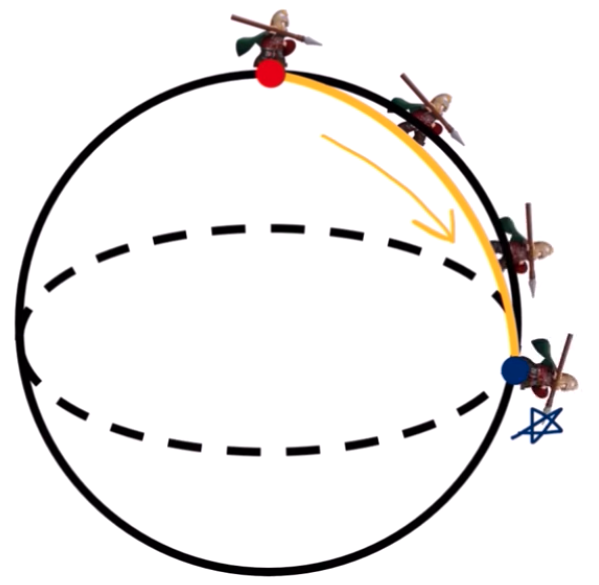
\includegraphics[scale=0.2]{figures/parallel-transport-01.png}
\end{center}

Of course, you can probably already see a problem with this parallel transport: if you imagine now, from the point 
of view of this person holding the arrow, traveling along the equator, always holding the arrow straight to him, and then 
walking backwards to the point it started on the north pole, you will find that the arrow/vector transported does not look like
when it started, so the starting and ending vectors are not the same:

\begin{center}
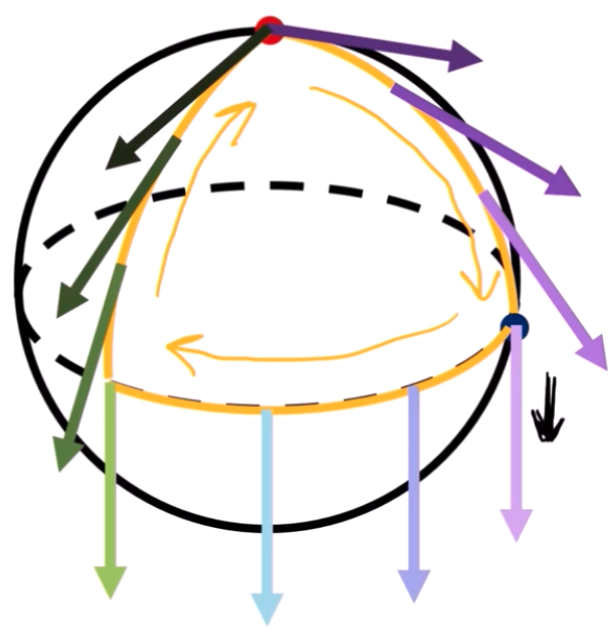
\includegraphics[scale=0.2]{figures/parallel-transport-02.png}
\end{center}

This means that \textbf{parallel transport DOES NOT keep vectors constant.}\\
The reason for that is that's \textbf{impossible to define a constant vector field on a curved surface.}\\
The parallel transport keeps vectors "as constant as possible" while moving along the surface step-by-step, and 
this is the best we can do, and the downside is that if traveling in a loop, we may and up
with a vector that looks differently than the one with started with.\\

Allright, now that we have the intuition, how do we describe this mathematically?
Referring to the last figure above, if we consider the first two vectors , the first at the north pole, and 
the next one moving towards the equator, and compare them, we can see that the change between them 
is this vector below, which points towards the center of the sphere, the same if we continue
comparing vectors in pair:

\begin{center}
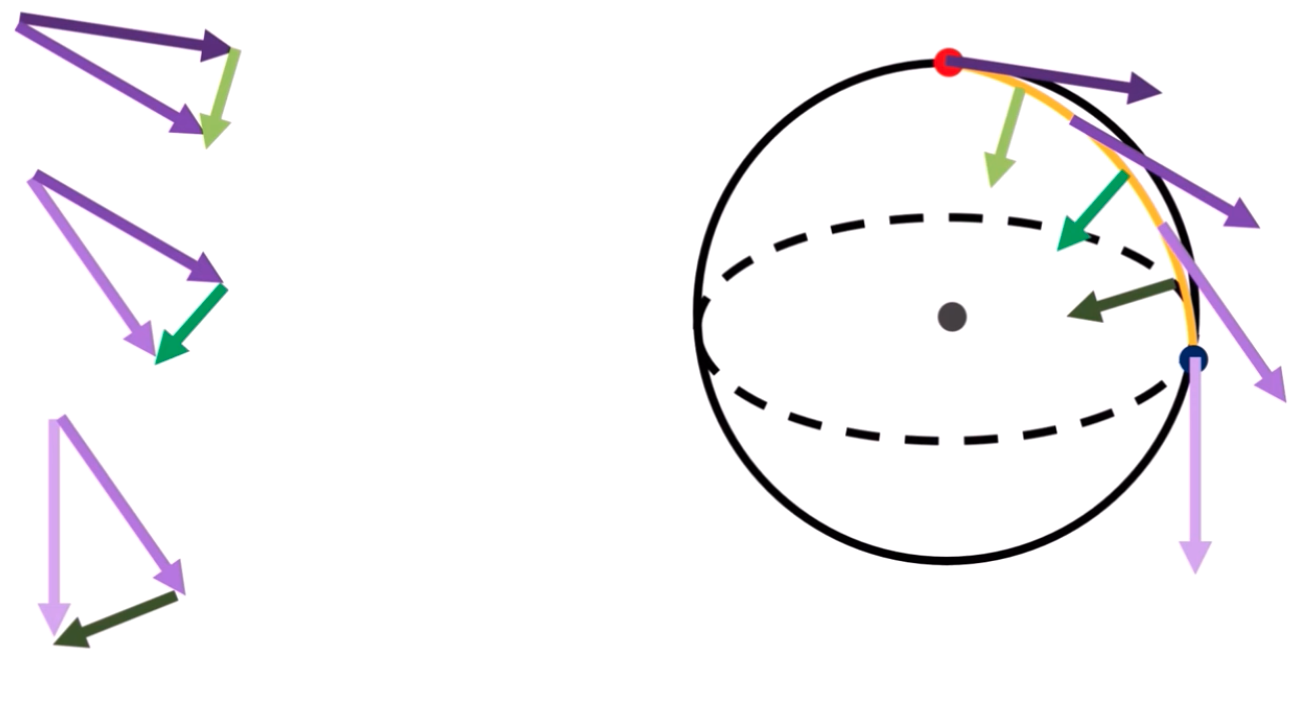
\includegraphics[scale=0.2]{figures/parallel-transport-03.png}
\end{center}

So this means that, when we parallel transport a vector "forward", its rate of change is completely normal to the surface,
perpendicular to the tangent plane.\\
Bringing this vector along this path, basically gives us a vector field defined at every point along this curve, and 
this vector field obeys this relationship:

\begin{equation}
    \frac{d \begingroup\color{violet}\vec{v}\endgroup}{d \begingroup\color{brown}\lambda\endgroup} = \begingroup\color{red}\vec{n}\endgroup
\end{equation}
 
Or, in other words, the difference between the rate of change of this vector field, and its normal part, is equal ot $\vec{0}$:

\begin{equation}
    \frac{d \begingroup\color{violet}\vec{v}\endgroup}{d \begingroup\color{brown}\lambda\endgroup} - \begingroup\color{red}\vec{n}\endgroup = \vec{0}
\end{equation}

So, the best that we can do to define a "constant" vector field on a curved surface, is parallel transporting a vector along
a curve, and this, is where the covariant derivative on curved surfaces come in.\\

\textbf{The covariant derivative on curved surfaces helps us find parallel transported vector fields.}\\

So we're going to define the covariant derivative on a curved surface, as the rate of change of a \textcolor{violet}{vector field} $\color{violet}\vec{v}$ in 
some \textcolor{teal}{direction} $\color{teal}\vec{w}$, with the \textcolor{red}{normal component, of the rate of change, subtracted.}.

\begin{equation}
    \nabla_{\begingroup\color{teal}\vec{w}\endgroup}\begingroup\color{violet}\vec{v}\endgroup
\end{equation}

So let's say we have a curve parametrized by the parameter $\color{brown}\lambda$, and as the parameter increases, we move forward along the curve. We have a vector field
$\color{violet}\vec{v}$ defined along this curve, and we want to find the rate of change of this vector field as we travel along the curve.\\

The covariant derivative of this vector field in a direction given by $d/d\lambda$, which is basically the direction 
along the curve, would be the rate of change of the vector field, in the lambda direction, with the component normal to the surface subtracted.

\begin{equation}
    \nabla_{\frac{d}{d\begingroup\color{brown}\lambda\endgroup}}\begingroup\color{violet}\vec{v}\endgroup = \frac{d\begingroup\color{violet}\vec{v}\endgroup}{d\begingroup\color{brown}\lambda\endgroup} - \begingroup\color{red}\vec{n}\endgroup
\end{equation}

And as we said, when this difference quantity is zero, it's when the vector field is being parallel transported along the curve.\\

So we can say that, when the covariant derivative $\nabla_{\begingroup\color{teal}\vec{w}\endgroup}\begingroup\color{violet}\vec{v}\endgroup = \vec{0}$, it means
that the vector field is parallel transported in the direction $\color{teal}\vec{w}$.\\

All of this can be clarified by giving an example, of the covariant derivative + parallel transport on a sphere of radius = 1.